%%%%%%%%%%%%%%%%%%%%%%%%%%%%%%%%%%%%%%%%%%%%%%%%%%%%%%%%%%%%%%%%%%%%%
%																	%
%	CHAPTER TWO, HARDWARE IN HPV									%
%																	%
%%%%%%%%%%%%%%%%%%%%%%%%%%%%%%%%%%%%%%%%%%%%%%%%%%%%%%%%%%%%%%%%%%%%%

\chapter{Hardware in HPC}

\section{Introduction}

Optimization can't be done without a good knowledge of the architecture of device, machine, or computer. 
Indeed, nowadays software and API try to take care of most of the optimizations but the last percents of gain always need to be architecture dependent. 
In this chapter we describe the most important devices architecures from classical processors, General Purpose Graphics Processing Units (GPGPUs), Field Programmable Gate Arrays (FPGAs) and Application-specific integrated circuits (ASICs).
Then those independants elements are use together in order to build supercomputers. 
The way they are arranged and the nodes interconnection is something that matters at large scale. 

\section{Architectures}
In this section we will describe the main nowadays architecture from HPC world and their specificities.

The CPU, as we know it today, begins its history with \textit{Texas Instruments Inc} and the first patent describing a CPU is "Computing systems cpu" proposed by \textit{Gary Boone} and published in 1973.
It is the reflection of the Von Neumann Machine we presented in Chapter I. 

From this first version plenty of optimizations arised. 
\begin{description}[noitemsep,nolistsep]
	\item[Multiple CPU cores] Multiple CPU cores on the same die. They can have independant or share part of the cache and access to the same main memory. The first machine were the IBM power4 with dual core.
	\item[In/Out-Of-Order] In-order-process is the one describes in previous chapter, the CU fetches instruction in memory, then the operands and the ALU computes, and finally the results is stored in memory. 
	In this model the time to perform an instruction, cumulation of instruction fetching + operand fetching + computation + store the resul, can be high and the ALU itself is busy only one step for computation itself. The idea of Out-of-order is to compute the instructions without following the PC order. Indeed, for independant tasks (this is know based on dependancy graphs) while the process fetch the next instructions data, the ALU can perform another operation with already available data. 
	\item[Prefetching] When a data is not available in L1 cache, it has to be moved from either L2 to L1 or L3 to L2 to L1 or in the worst case RAM to L3 to L2 to L1. Prefecthing technology is a way to, knowing the next instructions operands, prefetch the data in closer cache. The prefetch can either be hardware or software implemented and can concern data and even instructions.
	\item[Vectorization] Processors allows the instructions to be executed at the same time in a SIMD manner. If the same instruction is executed on coalescent data they can be executed in the same clock cycle. 
	Of course this tool require specific care during coding. 
\end{description}
Those optimizations can be found either in the classical processor model or accelerators.  

\subsection{Classical processors}

Nowadays processors share mostly the same architecture. 
They are called multi-cores and provide up to 2 to 16 cores and each constructor have its own specificities. 
Those processors are called "Host" because they are usually bootable and most of the accelerators need to be attached to them in order to work.

\subsubsection{Intel}

Intel was created in 1968 by a chemist and a physicists, Gordon E. Moore and Robert Noyce, in Montain View, California. 
Nowadays processors are mostly Intel ones, this world leader equips around 90\% of the supercomputers (November 2017 TOP500 list).
Since 2007 Intel adopted a production model called the "Tick Tock", presented on Fig.~\ref{fig:1_HPC:intel_tick_tock}.

\begin{figure}
\begin{center}
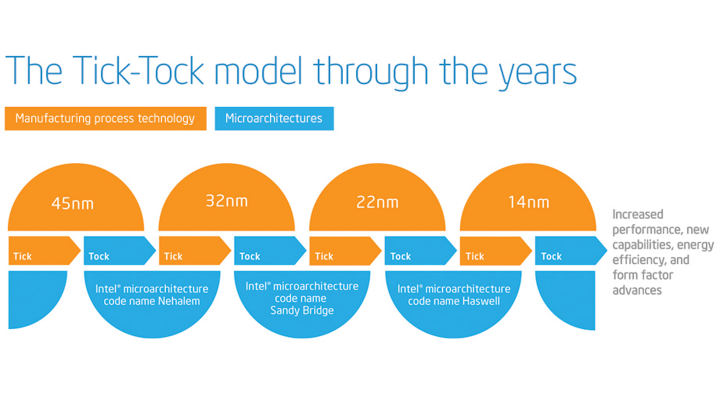
\includegraphics[width=.8\textwidth]{\locpath/figures/chap1/intel_tick_tock.png}
\caption{Intel Tick-Tock model}
\label{fig:1_HPC:intel_tick_tock}
\end{center}
\end{figure}

Since its creation the model followed the same fashion, a new manufacturing technology like shrink of the chip with better engraving on a "Tick" and a new microarchitecture delivered on a "Tock".
The Intel processors for HPC are called Xeon and features ECC memory, higher number of cores, large RAM support, large cache-memory, Hyperthreading, etc. compared to desktop processors. 
Every new processor have a code name. 
The last generations are chronologically called Westemere, Sandy Bridge, Ivy Bridge, Haswell, Broadwell, Skylake and Kaby lake. 
Kaby Lake, the last architecture of processor, does not exactly fit the usual "Tick-Tock" process because it is just based on optimizations of the Skylake architecture. 
It is produce like Skylake in 14nm.
This model seems to be hard to maintain due to the difficulties to engrave in less than 10nm with quantum tunneling. 

\subsubsection{Hyperthreading}
Another specificity of Intel processor is Hyperthreading (HT). 
This technology makes a single physical processor appearing as two logical processors for user's level.
In fact a processors embedding 8 cores will appear as a 16 cores for user. 
Adding more computation per node can technically allows the cores to switch context when data are fetched from the memory using the processor 100\% during all the computation. 
A lot of studies have been released on HT from Intel itself~\cite{marr2002hyperthreading} to other studies~\cite{bononi2006exploring,leng2002empirical}.
This does not fit to all the cases and can be disable for normal use of the processors. 

\subsubsection{Xeon Phi}
Another specific HPC product from Intel is the Xeon Phi. 
This device can be considered as a Host or Device/Accelerator machine. 
Intel describes it as "a bootable host processor that delivers massive parallism and vectorization".
This architecture embedded multiple multi-cores processors interconnected. 
This is call Intel's Many Integrated Core (MIC).
The architectures names are Knights Ferry, Knights Ferry, Knights Corner and Knight Landing~\cite{sodani2016knights}. 
The last architecture, Knight Hill, was recently canceled by Intel. 
The main advantage of this architecture compared to GPGPUs is the x86 compatibility of the embedded cores and the fact this device can boot and use to drive other accelerators. 
They also feature more complex operations and handle double precision natively. 

\subsubsection{ARM}
Back in 1980s, ARM stood for Acorn RISC Machine in reference of the first company implementing this kind of architecture, Acorn Computers. 
This company later changed to Advanced RISC Machine (ARM). 
ARM is a specific kind of CPU based on RISC architecture as its ISA depsite usual processors using CISC.
The downside of CISC machines makes them hard to create and they require way more energy to work. 
The ISA from the RISC is simplier and requires less transistors to operate. 
Therefore, the energy required and the heat dissipated is less important. 
It would then be easier to create massively parallel processors based on ARM. 
On the other hand, simple ISA impose more work on the source compilation to fit the simple architecture. 
That makes the instructions sources longer and therefore more single instructions to execute. 

The ARM company provide several version of ARM processors named Cortex-A7X, Cortex-A5X and Cortorx-A3X respectively balancing highest-performances, performances and efficiency and less power consumption. 
We find here the same kind of naming as Intel processors. 

The new ARMv8 architecture starts to have the tools to target HPC context~\cite{rico2017arm}.
The european approach towards energy efficient HPC, Mont-Blanc project\footnote{http://montblanc-project.eu/}, already constructs ARM based supercomputers. 
For the Exascale project in Horizon 2020 this project focus on using ARM-based systems for HPC with many famous contributors with Atos/Bull as a project coordinator, ARM, French Alternative Energies and Atomic Energy Commission (CEA), Barcelona Supercomputing Center (BSC), etc.
The project is decomposed in several steps to finaly reach Exascale near 2020. 
The third step, Mont-Blanc 3, is about to work on a pre-exascale prototype powered by Cavium’s ThunderX2 ARM chip based on 64-bits ARMv8.

\subsection{GPGPU}

GPUs are based on the SIMD model of the Flynn taxonomy presented previously, \emph{Single Instruction, Multiple Data}.
The specific execution model is called SIMT (\emph{Single Instruction, Multiple Thread}). It enables the execution of millions of coordinated threads in a data-parallel mode. 
Two main companies provide GPGPUs for HPC: NVIDIA and AMD.
We will present them in that order and conclude on the differences. 

\subsubsection{NVIDIA GPU architecture}

The NVIDIA company was fonded in April 1993 in Santa Clara, Carolina, by three persons in which Jensen Huang, the actual CEO.
Its name seems to come from \textit{invidia} the latin word for Envy and vision, for the graphics generation. 

Known as the pioner in graphics, cryptocurrency, portable devices and now AI, it seems to be even the creator of the name "GPU".
It GPU, inspired from visualisation and gaming at a first glance, is available as a dedicated device  since the Tesla. 
The public GPUs can also be use for dedicated computation but does not feature ECC memory, double precision or special functions/FFT cores. 

\begin{figure*}[t!]
\centering
\setlength\fboxsep{0pt}
\setlength\fboxrule{0.25pt}
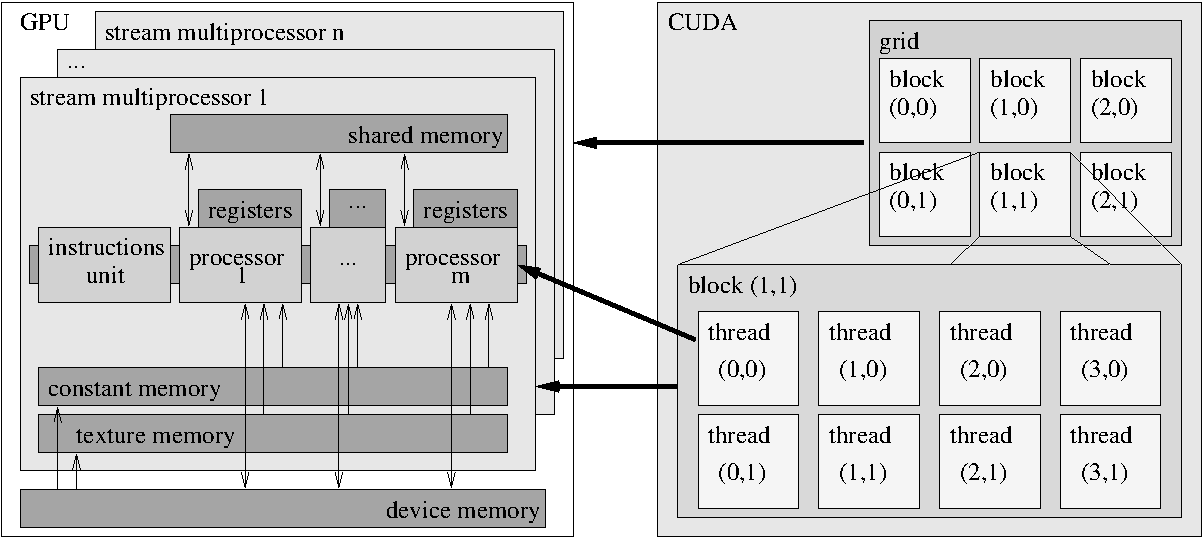
\includegraphics[scale=0.6]{\locpath/figures/chap1/smx}
\caption{NVIDIA GPU and CUDA architecture overview}
 \label{fig:chap1_gpu}
%\vspace{-0.8cm} 
\end{figure*}

As presented in Fig.\ref{fig:chap1_gpu}, NVIDIA GPUs include many \emph{Streaming Multiprocessors} (SM), each of which is composed of many \emph{Streaming Processors} (SP). In the Kepler architecture, the SM new generation is called SMX.
%
%In the CUDA programing model~\cite{cuda}, the GPU works as a SIMT co-processor of a conventional CPU. 
Grouped into \emph{blocks}, \textit{threads} execute \emph{kernel} functions synchronously.
Threads within a block can cooperate by sharing data on an SMX and synchronizing their execution to coordinate memory accesses; inside a block, the scheduler organizes \emph{warps} of 32 threads which execute the instructions simultaneously.
The blocks are distributed over the GPU SMXs to be executed independently.

\subsubsection{Memory, bandwidth and streams:}

In order to use data in a CUDA kernel, it has to be first created on the CPU, allocated on the GPU and then transferred from the CPU to the GPU; after the kernel execution, the results have to be transferred back from the GPU to the CPU. 
GPUs consist of several memory categories, organized hierarchically and differing by size, bandwidth and latency.   
On the one hand, the device's main memory is relatively large but has a slow access time due to a huge latency. 
On the other hand, each SMX has a small amount of shared memory and L1 cache, accessible by its SPs, with faster access, and registers organized as an SP-local memory. 
SMXs also have a constant memory cache and a texture memory cache.
%, that are linked to the constant and texture memories physically located in the device memory: these are read-only and have faster access time than the rest of the memory categories.
Reaching optimal computing efficiency requires considerable effort while programming.
Most of the global memory latency can then be hidden by the threads scheduler if there is enough computational effort to be executed while waiting for the global memory access to complete. Another way to hide this latency is to use streams to overlap kernel computation and memory load. 

\subsubsection{Threads synchronization:}
It is also important to note that branching instructions may break the threads synchronous execution inside a warp and thus affect the program efficiency. 
This is the reason why test-based applications, like combinatorial problems that are inherently irregular, are considered as bad candidates for GPU implementation. 
%This is particularly true with regard to combinatorial problems resolution. 
Thus we intend to provide a way to regularize their execution, in order to get good acceleration with GPU computation. 

\subsubsection{HPC tools}
Specific tools have been made for HPC in the NVIDIA GPGPUs. 
\begin{description}[noitemsep,nolistsep]
	\item[Dynamic Parallelism] This feature allow the GPU kernels to run other kernels themself. This feature 
	\item[Hyper-Q] This technology enable several CPU threads to execute kernels on the same GPU simultaneously. This can help to reduce the synchronization time and idle time of CPU cores for specific applications.
	\item[NVIDIA GPU-Direct] GPUs' memory and CPU ones are different and the Host much push the data on GPU before allowing it to compute. GPU-Direct allows direct transferts from GPU devices through the network. Usually implemented using MPI.  
\end{description}

We give details on the GPU we mainly used in this study in the ROMEO supercomputer center. 

\subsubsection{Details on K20X}
This NVIDIA Tesla Kepler GPU is based on the GK110 graphics processor describes in the whitepaper\cite{nvidia2012nvidias} on 28nm process.
This GPU comes in active and passive cooling with respectively K20Xc and K20Xm.
This GPU embedded 2688 CUDA cores distributed in 14 SMX (we note that GK110 normally provides 15 SMX but only 14 are present4 on the K20X).
This GPU features 

\todo{Describe K20Xm, 2688 cores}


\subsection{AMD}
Another company is providing GPUs for HPC, Advanced Micro Devices (AMD). 
In front of the huge success of NVIDIA GPU that leads from far the HPC market, it is hard for AMD to place its GPGPUs. 
Their HPC GPUs are called FirePro.
They are targeting using a language near CUDA called OpenCL. 

\subsection{FPGA and ASIC}
Field Programmable Gates Array are device that can de reprogram to fit the needs of the user after their construction.
The leader was historically Altera with the Stratix, Arria and Cyclone FPGAs and is now part of Intel. 
With the FPGAs the user have access to the hardware itself and can design its own circuit. 
Nowadays FPGA can be targeted 

ASICs are dedicated device construct for on purpose. 
An example of ASIC can be the Gravity Pipe (GRAPE) which is dedicated to compute gravitation given mass/positions.
Google leads the way for ASIC and just created its dedicated devices to boost AI bots. 

\section{Interconnection and clusters}

\subsection{Interconnects}
Interconnect is the way the nodes of a cluster are connected together. 
Several topologies exists from point to point to multi dimensional torus.
The most commons are references in Fig

InfiniBand (IB) is the most spread technology used for interconnect with different kind of bandwith.
\begin{figure}
\begin{center}
\[\arraycolsep=0.pt\def\arraystretch{1.2}
\begin{tabular}{| l | l | l | l | l | l | l | l |}
\hline
Name & Single DR & Double DR & Quad DR & Fourth DR & Enhanced DR & Highg DR & Next DR \\
\hline
Rate (Gbs) & 2.5 & 5 & 10 & 14.0625 & 25.78125 & 50 & 100 \\
\hline
Year & 2003 & 2005 & 2007 & 2011 & 2014 & 2017 & 2020 \\
\hline
\end{tabular}
\]
\end{center}
\end{figure}


\subsection{TOP500 remarquable clusters}
\subsubsection{Sunway Taihulight}

Sunway Taihulight is the third Chinese supercomputer to be ranked in the first position of the TOP500 list. \todo{(VERIFIER)}
A recent report from Jack Dongarra, a figure in HPC, decrypt the architecture of this supercomputer\cite{dongarra2016report}. 
The most interessant point is the conception of this machine, completely done in China. 
The Sunway CPUs were invented and built in China, the Vendor is the Shanghai High Performance IC Design Center. 

\begin{figure}
\centering
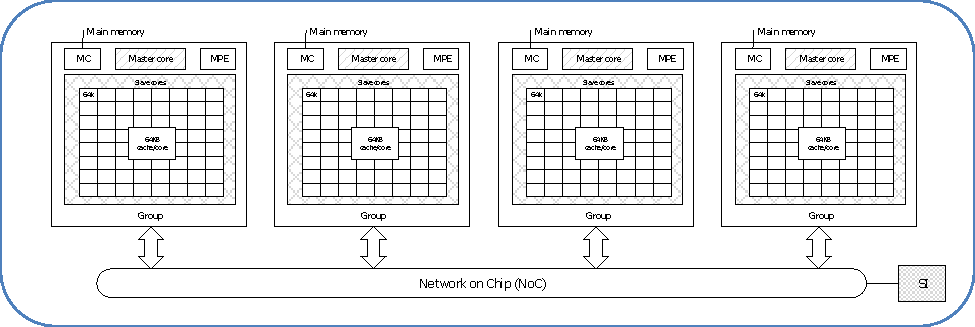
\includegraphics[scale=1]{\locpath/figures/Chap1/report_sunway_CPE}
\caption{Sunway Taihulight node architecture from \textit{Report on the Sunway TaihuLight System}, Jack Dongarra, June 24, 2016.}
\label{fig:chap1_report_sunway_CPE}
\end{figure}

The SW26010, a many core architecture, features 260 cores based on RISC architecture and a specific conception depicted on Fig.\ref{fig:chap1_report_sunway_CPE}.

\subsubsection{Piz Daint}
The supercomputer of the CSCS, Swiss National Supercomputing Center, is currently ranked 2nd of the November 2017 TOP500 list. 
This GPU accelerated GPU is a most powerful representative of the  

\subsubsection{K-Computer}
K-Computer was the top 1 supercomputer of TOP500 2011 list. 

The TOFU interconnect network makes the K-Computer unique~\cite{ajima2009tofu} and stands for TOrus FUsion.
This interconnect mixes a 6D Mesh/Torus interconnect to provide up to  ...

\subsubsection{Sequoia/Mira}
Sequoia supercomputer was top 1 of the TOP500 2012 list. 
It is based on BlueGene from IBM.
The BlueGene project made up to three main architectures with BlueGene/L, BlueGene/P and BlueGene/Q.

\section{ROMEO Supercomputer}

The ROMEO supercomputer center is the computation center of the Champagne-Ardenne region in France. 
Hosted since 2002 by the University of Reims Champagne-Ardenne, this so called meso-center (French name for software and hardware architectures) is used for HPC for theoric research and domain science like applied mathematics, physics, biophysics and chemistry. 

This project is support by the Champagne-Ardenne region and the CEA (French Alternative Energies and Atomic Energy Commission), aim to host research and production codes of the region for industrial, research and academics purposes. 

We are currently working on the third version of ROMEO, installed in 2013. 
As many of our tests in this study have been done on this machine, we will carefully describe its architecture. 

This supercomputer was ranked 151st in the TOP500 and 5th in the GREEN500 list. 

\subsection{ROMEO hardware architecture}
ROMEO is a Bull/Atos supercomputer composed of 130 BullX R421 computing nodes. 

Each node is composed of two processors Intel Ivy Bridge 8 coeurs @ 2,6 GHz. 
Each processor have access to 16GB of memory for a total of 32GB per node, the total memory if 4.160TB. 
Each processor if linked, using PCIe-v3, to an NVIDIA Tesla K20Xm GPGPU. 
This cluster provide then 260 processors for a total of 2080 CPU cores and 260 GPGPU providing 698880 GPU cores. 
The computation nodes are interconnected with an Infiniband QDR non-blocking network structured as a FatTree. 
The Infiniband is a QDR providing 10GB/s. 

The storage for users is 57 TB and the cluster also provide 195 GB of Lustre and 88TB of parallel scratch filesystem. 

In addition to the 130 computations nodes, the cluster provides a visualization node NVIDIA GRID with two K2 cards and 250GB of DDR3 RAM. 
The old machine, renamed Clovis, is always available but does not features GPUs. 

The supercomputer supports MPI with GPU Aware and GPUDirect. 
